\section{Introduction}

\subsection{ATLAS}

\begin{frame}
	\begin{center}
	\Large{Introduction}
	\end{center}
\end{frame}

%\begin{frame}
%	\frametitle{The Higgs Boson}
%	%\begin{columns}
%	%\column[c]{.60\textwidth}
%	The Higgs mechanism allows certain particles to acquire mass.
%	\begin{itemize}
%		\item Existence predicted in 1964.
%		\item Incorporated into Standard Model in 1967.
%		\item Discovered with the experiments CMS and ATLAS in 2012.
%	\end{itemize}
%	%\column[c]{.50\textwidth}
%	    %
\includegraphics[width=130pt]{images/higgs_logo}
%	%\end{columns}	
%\end{frame}

\begin{frame}
	\frametitle{A Toroidal LHC ApparatuS (ATLAS)}
	\begin{columns}
	\column[t]{.50\textwidth}
	\begin{itemize}
		\item Registers $\sim$40 million particle collisions (called events) per second.
		\item Aims to investigate four major topics in physics.
		\item Discovered the Higgs Boson in 2012.
		\item Tests predicted properties of the Higgs boson.
	\end{itemize}
	\column[t]{.50\textwidth}
	\begin{figure}
		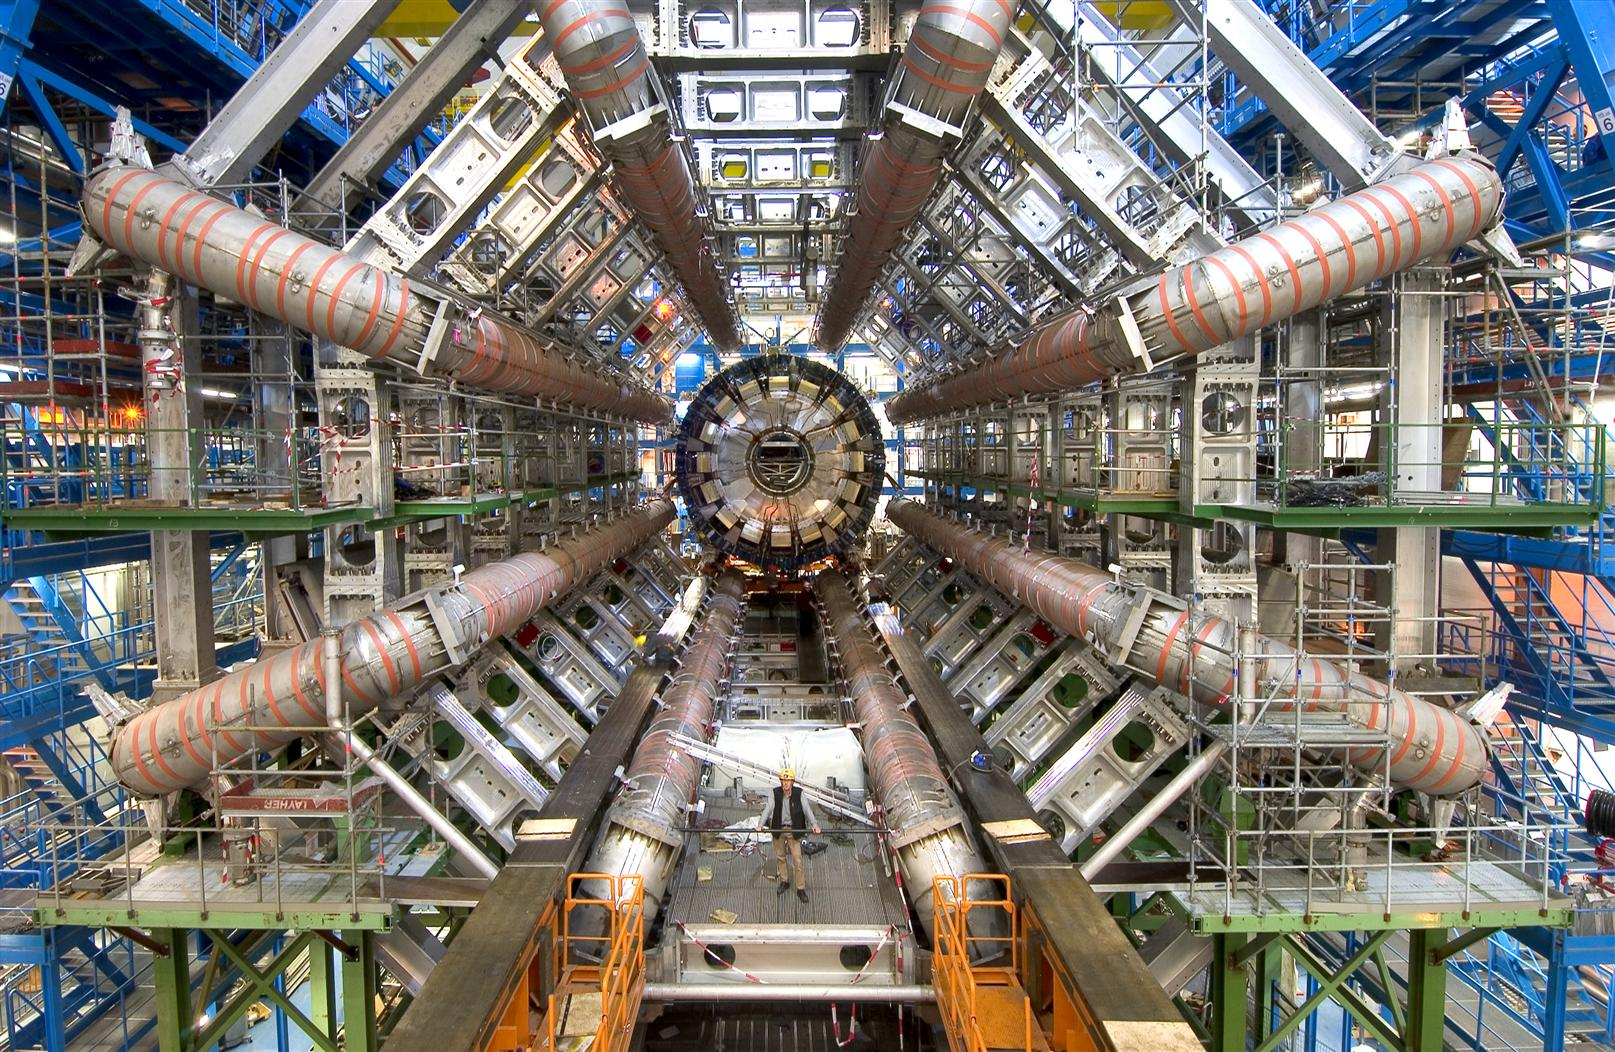
\includegraphics[width=\linewidth]{images/atlasgross}
		\caption{\raggedleft The ATLAS detector. \cite{atlasHP}}
	\end{figure}
	\end{columns}
\end{frame}

\subsection{Data processing of ATLAS}
\begin{frame}
	\frametitle{Data processing of ATLAS}
	\begin{itemize}
		\item Three levels of filtering, reducing events from 40 million to 200 per second. (The \emph{trigger})
		\item Regions in feature space are picked for further analysis. They are called the \emph{selection region}.
		\item Recorded and compressed events that are part of this region are reconstructed for the current task.
	\end{itemize}
	\begin{flushright}
	\cite{atlasHP}
	\end{flushright}
\end{frame}